
El presente capítulo tiene por objetivo describir los principales conceptos asociados a la formación de complejos proteicos y a su predicción, facilitando al lector la comprensión de las secciones posteriores.


\section{Ambiente de Desarrollo de Ingeniería de Software}
\subsection{Metodología de Desarrollo}

La metodología de desarrollo a utilizar en el proyecto es ... 
Esta metodología fue seleccionada ya que este proyecto ...
este software ...

\subsection{Tecnologías Utilizadas (Backend, Frontend, Base de Datos)}



\subsection{Estándares de Documentación}

Adaptación basada en IEEE Software Test Documentation Std 829-1998 
Adaptación basada en IEEE Software Requirements Specifications Std 830-1998

\subsection{Técnicas y notaciones}

ejemplo: Diagramas de Casos de Uso -notación UML es utilizada para detallar la funcionalidad del software 

\subsection{Herramientas, framework, lenguaje usados en el desarrollo del proyecto}

ejemplo: MongoDBCompass versión 1.33.0, herramienta utilizada para la consulta de las estructuras de datos -collections

\section{Especificación de requerimientos - Producto SW}
\subsection{Límites}

El software / app no permitirá ...

\subsection{Rectricciones Técnicas}

La empresa cuenta con ...

\subsection{Objetivo General y Especificos de SW}

\subsubsection{Objetivo General}

Defina sólo 1 objetivo general. Utilice 1 verbo activo que englobe la contribución o aporte del software completo en la empresa. Todos los objetivos de software se escriben así: El sistema HACE ALGO con lo que la empresa REDUCE COSTOS/ AUMENTA  INGRESOS/ AUMENTA UTILIDAD 
Por ejemplo: El sistema manejará información del proceso de postulación de a cargos para que la empresa optimice el uso de los recursos utilizados en el proceso, es decir reduciendo los recursos gastados por todos los involucrados en el registro, evaluación y resultados.

\subsubsection{Objetivos Especificos de SW}

Utilice 1 verbo activo que contribuya al objetivo general, es decir la contribución de ciertas funciones del software en la empresa. Todos los objetivos de software se escriben así: El sistema HACE ALGO con lo que la empresa REDUCE COSTOS/ AUMENTA  INGRESOS/ AUMENTA UTILIDAD. Por Ejemplo: 
\begin{itemize}
    \item El sistema permite que los postulantes sean notificados directamente, se mantengan todos informados de las etapas y actividades a realizar, de esta forma la empresa elimina el tiempo de la secretaria en confirmaciones telefónicas o agenda de entrevistas.
    \item El sistema permite que las postulaciones sean realizadas por los postulantes y solo aquellas que cumplen con los requisitos obligatorios sean revisadas por el comité, de esta forma la empresa elimina el tiempo de la secretaria y de la comisión revisando curriculum incompletos.
\end{itemize}

\subsection{Planificación de reuniones con usuarios}
\subsection{Requerimientos Funcionales}

La lista de los requerimientos funcionales específicos se presenta en la Tabla 10.
• Los \begin{itemize}
    \item requerimientos pueden ser agrupados por distintos criterios, por ejemplo, tipo de usuario o módulo (otras organizaciones se encuentran en el anexo del estándar IEEE Std 830-1998).
    \item Se recomienda el uso de la forma verbal en infinitivo para denotar las acciones que el software debe realizar.
    \item Los requerimientos deben ser enumerados para facilitar su seguimiento. 
    \item En la descripción de cada requerimiento se incluyen condiciones o restricciones del requerimiento, por ejemplo “los registros de los clientes pueden ser eliminados si y sólo si el cliente no ha efectuado ninguna compra en los 5 últimos años”. 
    \item Los requerimientos de su proyecto considerando se redactan contestando, al menos, las preguntas: Quien, Que, Que restricciones existen, Cuando, Que pasa después? Por ejemplo: 
    
    El CLIENTE o la ENCARGADA de recepción pueden REGISTRAR reserva de habitaciones, el cliente NO REQUIERE estar registrado y puede reservar COMO MÁXIMO 10 habitaciones a través de la web. La encargada de recepción puede reservar MÁS DE 10 habitaciones con la autorización del Encargado de Administración. Se puede registrar reserva SÓLO SI EXISTE DISPONIBILIDAD en fecha y habitaciones. El registro EXITOSO genera un código de reserva, y la reserva que queda en estado no confirmada.
    \item Sino se especifican los requisitos contestando a las preguntas no será evaluado
\end{itemize} 

 \begin{table}[H]
    \begin{center}
        \begin{tabular}{ | m{2cm} | m{9cm} | }
            \hline \textbf{id} & \textbf{el sistema debe }\\ \hline
            RF\_01 &   \\ \hline
            RF\_02 &     \\ \hline
              &    \\ \hline
        \end{tabular}
        \caption{Requerimientos Funcionales}
    \end{center}
\end{table}

\subsection{Requerimientos No Funcionales}

Misma idea de arriba

\subsection{Interfaces externas de Entrada}

Cada interfaz externa, es una especificación tomada desde IEEE Std 830-1998 página 22, tal como lo muestra la figura. Se separa en ENTRADA Y SALIDA.

\begin{figure}[H]
    \centering
    
\includegraphics[scale=0.5]{figures/i1.png}
    \caption{Ejemplo1}
    \label{fig:e1}
\end{figure}

\begin{figure}[H]
    \centering
    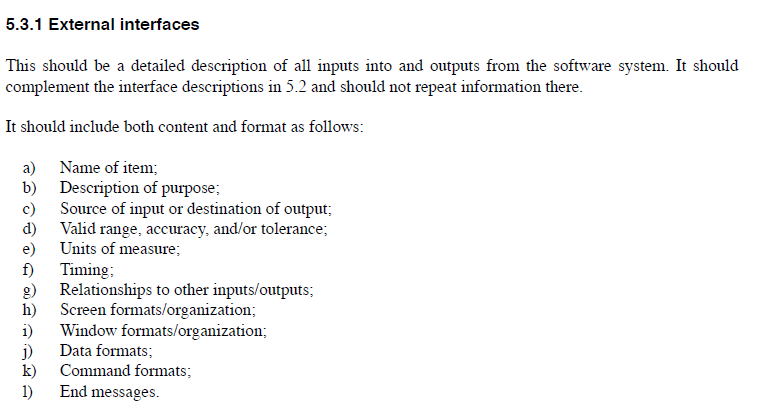
\includegraphics[scale=0.5]{figures/i2.png}
    \caption{Ejemplo2}
    \label{fig:e2}
\end{figure}

Interfaz externa de entrada, es decir un conjunto de datos que serán ingresados al sistema independiente del medio de ingreso, es decir datos que provienen de un usuario a través de teclado, lector de código barra, etc.
En la tabla se incluyen los ítems de datos 1 sola vez, por ejemplo, no es necesario repetir el rut del proveedor o el código del producto, en esta tabla importan QUE DATOS INGRESARÁN y no importa cuántas veces ingresen.

 \begin{table}[H]
    \begin{center}
        \begin{tabular}{ | m{2cm} | m{3cm} | m{9cm} |}
            \hline \textbf{Identificador} & \textbf{Nombre del ítem} & \textbf{Detalle de Datos contenidos en ítem} \\ \hline
            Ejemplo: 
            DE\_01 & Datos del proveedor  & NOMBRE, RUT\_PROV, GIRO, DIRECCION,TELEFONO ...\\ \hline
            DE\_02 & Datos de factura & RUT\_PROV,FECHA\_FACT, TIPO\_PAGO, COD\_PROD, CANT\_COMPRADA, PRECIO …….   \\ \hline
            DE\_03 & Datos de productos & COD\_PROD, NOMBRE   \\ \hline
                  &        & \\ \hline
        \end{tabular}
        \caption{Interfaces de Entrada}
    \end{center}
\end{table}

\subsection{Interfaces externas de Salida}

Se especifica cada salida del sistema, conjuntos de datos que se sacan del sistema para los usuarios u otros sistema,  indicando en cada caso el formato o medio de salida. 


 \begin{table}[H]
    \begin{center}
        \begin{tabular}{ | m{2cm} | m{3cm} | m{8cm} | m{2cm} |}
            \hline \textbf{Identificador} & \textbf{Nombre del ítem} & \textbf{Detalle de Datos contenidos en ítem} & \textbf{Medio Salida}\\ \hline
            Ejemplo: 
            IS\_01 & Informe de los proveedores  & NOMBRE, RUT, CODIGO,GIRO,DIRECCION,TELEFONO & Archivo XLS, Impresora, Pantalla\\ \hline
             &  &  & \\ \hline
             &  &  & \\ \hline
             &  &  & \\ \hline
        \end{tabular}
        \caption{Interfaces de Salida}
    \end{center}
\end{table}

\section{Factibilidad del Proyecto}
\subsection{Factibilidad Técnica}

Describa si:
\begin{itemize}
    \item Existen las personas para construir el software, si las personas tienen los conocimientos y competencias técnicas.
    \item Existen o se pueden adquirir sw de desarrollo y necesario para explotación del sw
    \item Existen o se pueden adquirir Hw de desarrollo (pc y server) y necesario para explotación del sw (server)
\end{itemize}




 \begin{table}[H]
    \begin{center}
        \begin{tabular}{ | m{5cm} | m{6cm} | }
            \hline \textbf{REQUERIMIENTOS} & \textbf{DESCRIPCIÓN }\\ \hline
            Sistema operativo   & Ubuntu 20.04 o superior. \\ \hline
            Procesador          & Pentium silver. \\ \hline
            Memoria RAM         & 4 GB. \\  \hline
            Espacio de almacenamiento & 2 GB.\\\hline
            Navegador           & safari, Opera, etc.\\ \hline
            Resolución de pantalla &  1280 x 768 px.\\ \hline
            Conexión a internet & Requerida.\\ \hline
        \end{tabular}
        \caption{Especificación de Software requerido en desarrollo del proyecto}
    \end{center}
\end{table}


 \begin{table}[H]
    \begin{center}
        \begin{tabular}{ | m{5cm} | m{6cm} | }
            \hline \textbf{REQUERIMIENTOS} & \textbf{DESCRIPCIÓN }\\ \hline
            XX & XX  \\ \hline
            XX & XX  \\ \hline
        \end{tabular}
        \caption{Especificación de Hardware requerido en desarrollo del proyecto}
    \end{center}
\end{table}


 \begin{table}[H]
    \begin{center}
        \begin{tabular}{ | m{5cm} | m{6cm} | }
            \hline \textbf{REQUERIMIENTOS} & \textbf{DESCRIPCIÓN }\\ \hline
            XX & XX  \\ \hline
            XX & XX  \\ \hline
        \end{tabular}
        \caption{Especificación de Hardware Servidor requerido en desarrollo del proyecto}
    \end{center}
\end{table}


Concluya si todo existe o se puede adquirir, o hay una comunidad de apoyo ... es técnicamente factible.


\subsection{Factibilidad Operativa}

Describa si:
\begin{itemize}
    \item Los clientes reconocen la importancia del sw y sus beneficios.
    \item Los usuarios reconocen la importancia del sw y sus beneficios.
    \item Los usuarios están disponibles a participar, tienen las competencias mínimas requeridas
\end{itemize}
Si lo anterior existe, o usted tomará las medidas para reforzarlo, entonces es operativamente factible.


\subsection{Factibilidad Económica}
Describa:

 \begin{table}[H]
    \begin{center}
        \begin{tabular}{ |l|l|l| }
            \hline 
            \textbf{Software} & \textbf{Licencia} & \textbf{Costo Licencia}\\ \hline
            XX & XX & XX  \\ \hline
            XX & XX & XX \\ \hline
        \end{tabular}
        \caption{Licencias}
    \end{center}
\end{table}

 \begin{table}[H]
    \begin{center}
        \begin{tabular}{ |l|l|l| }
            \hline 
            \textbf{Item} & \textbf{\$ mensual aprox. en CLP} & \textbf{\$ anual aprox. en CLP}\\ \hline
            XX & XX & XX  \\ \hline
            XX & XX & XX \\ \hline
        \end{tabular}
        \caption{Costo hosting y dominio, Este servicio tiene un costo anual obtenido de https://www.nic.cl/dominios/tarifas.html}
    \end{center}
\end{table}

\begin{table}[H]
    \begin{center}
        \begin{tabular}{ |m{2cm}|m{2cm}|m{5cm}|m{5cm}| }
            \hline 
            \textbf{Recurso Humanos} & \textbf{Cantidad personal} & \textbf{Sueldo aprox. en CLP por mes} &
            \textbf{Sueldo aprox. en CLP por duración proyecto (x meses)}\\ \hline
            XX & XX & XX & XX \\ \hline
            XX & XX & XX & XX\\ \hline
        \end{tabular}
        \caption{ Calculo costo de desarrollo y soporte.}
    \end{center}
\end{table}

\subsubsection{Flujo de caja}

Para asegurar la viabilidad económica del proyecto, se empleará el indicador del Valor Actual Neto (VAN) como medida. Para ello, se realizará el cálculo del flujo de caja correspondiente a la inversión inicial, así como se proyectarán los flujos de caja para los primeros 5 años. Estos datos se presentan en detalle en la siguiente tabla:

\begin{table}[H]
    \begin{center}
        \begin{tabular}{ |m{2cm}|m{2cm}|m{1cm}|m{1cm}|m{1cm}|m{1cm}|m{1cm}| }
            \hline 
            \textbf{Recurso Humanos} & \textbf{Año 0} & \textbf{Año 1} &
            \textbf{Año 2} & \textbf{Año 3} & \textbf{Año 4} & \textbf{Año 5} \\ \hline
            (+) Ingresos &  &  &  &  &  & \\ \hline
            Beneficios   & \$ costo desarrollo (ahorro) \$ reducción de costos
            (ahorro) & XX & XX & XX & XX & XX\\ \hline
            (-) Costos   &  &  &  &  &  & \\ \hline
            &  &  &  &  &  &\\ \hline
            Servicios & (\$b) & (\$b) & (\$b) & (\$b) & (\$b) & (\$b)\\ \hline
            Soporte y Mantención & (\$a) & (\$a) & (\$a) & (\$a) & (\$a) & (\$a)\\ \hline
            TOTAL & (\$ab) & (\$ab) & (\$ab) & (\$ab) & (\$ab) & (\$ab)\\ \hline
        \end{tabular}
        \caption{ Calculo costo de desarrollo y soporte.}
    \end{center}
\end{table}


\subsubsection{Cálculo del V.A.N}

Donde cada uno de los términos, se especifican en la Tabla:


 \begin{table}[H]
    \begin{center}
        \begin{tabular}{ | m{2cm} | m{8cm} | }
            \hline \textbf{Término} & \textbf{Significado }\\ \hline
            $t$ & Intervalo de tiempo   \\ \hline
            $n$ & Duración en años  \\ \hline
            $I_0$ & Inversión inicial $(t=0)$   \\ \hline
            $K$ & Tasa de descuento   \\ \hline
            $Vt$ & Flujos de caja obtenidos en el intervalo de tiempo $t$   \\ \hline
        \end{tabular}
        \caption{Términos de la fórmula de VAN}
    \end{center}
\end{table}

A continuación, se calculará el VAN con una tasa de descuento del 10%.

 \begin{table}[H]
    \begin{center}
        \begin{tabular}{ | m{5cm} | m{6cm} | }
            \hline \textbf{Año} & \textbf{Flujo de Caja }\\ \hline
            \textbf{Año 0} & $\$ab/(1+0.10)^0 = \$$  \\ \hline
            \textbf{Año 1} & $\$ab/(1+0.10)^1 = \$$  \\ \hline
            \textbf{Año 2} & $\$ab/(1+0.10)^2 = \$$  \\ \hline
            \textbf{Año 3} & $\$ab/(1+0.10)^3 = \$$  \\ \hline
            \textbf{Año 4} & $\$ab/(1+0.10)^4 = \$$  \\ \hline
            \textbf{Año 5} & $\$ab/(1+0.10)^5 = \$$  \\ \hline
        \end{tabular}
        \caption{Cálculo del VAN}
    \end{center}
\end{table}

$ VAN (10\%) = Año 0 + Año 1 + Año 2 + Año 3 + Año 4 + Año 5 $

$             = \$ $

$ VAN (10\%) = \$ $


En este caso, el VAN obtenido es positivo (\$   ), lo que indica que el proyecto es viable desde una perspectiva económica.

\subsection{Conclusión de Factibilidad}

Gracias al análisis realizado en los puntos anteriores, se puede concluir que el proyecto es 
